% 2.5D heterogeneous integration on a passive interposer (scope diagram).
% Adapted from the ESTC 2026 paper figure fig_25d_interposer.tex (same project).
\documentclass[border=3mm]{standalone}
\usepackage{tikz}
\usetikzlibrary{arrows.meta}
\usepackage[T1]{fontenc}
\usepackage{lmodern}

\definecolor{IHPfg}{RGB}{0,80,139}
\definecolor{IHPaccent}{RGB}{109,112,114}
\definecolor{cInterposer}{RGB}{0,80,139}
\definecolor{cDieA}{RGB}{55,135,190}
\definecolor{cDieB}{RGB}{210,80,80}
\definecolor{cCuPillar}{RGB}{184,115,51}
\definecolor{cPackage}{RGB}{160,160,165}

\begin{document}
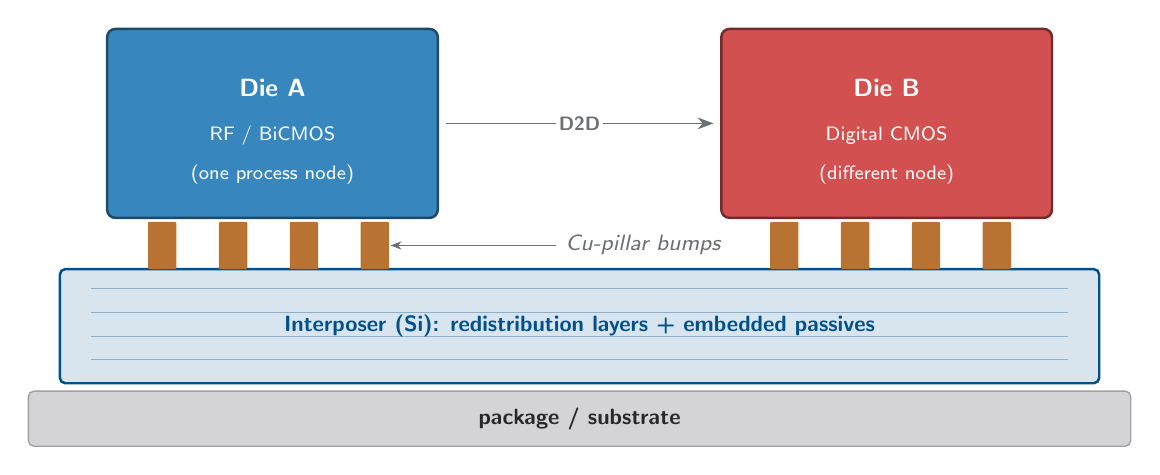
\begin{tikzpicture}[
    dielbl/.style={font=\sffamily\small\bfseries, text=white, align=center},
    diesublbl/.style={font=\sffamily\scriptsize, text=white, align=center},
    layerlbl/.style={font=\sffamily\footnotesize\bfseries},
    notelbl/.style={font=\sffamily\footnotesize\itshape, text=IHPaccent}
]

% --- PACKAGE / SUBSTRATE (bottom strip) ---
\fill[cPackage!45, draw=cPackage, line width=0.5pt, rounded corners=2pt]
    (0, -0.7) rectangle (14, 0.0);
\node[layerlbl, text=cPackage!25!black]
    at (7, -0.35) {package / substrate};

% --- INTERPOSER ---
\fill[cInterposer!15, draw=cInterposer, line width=0.9pt, rounded corners=2pt]
    (0.4, 0.10) rectangle (13.6, 1.55);
% RDL routing hint (light horizontal lines inside the interposer)
\foreach \y in {0.40, 0.70, 1.00, 1.30} {
    \draw[cInterposer!45, line width=0.35pt] (0.8, \y) -- (13.2, \y);
}
\node[layerlbl, text=cInterposer]
    at (7, 0.83) {Interposer (Si): redistribution layers + embedded passives};

% --- Cu PILLAR BUMPS (under each die) ---
\foreach \x in {1.7, 2.6, 3.5, 4.4} {
    \fill[cCuPillar, rounded corners=0.4pt]
        (\x-0.18, 1.55) rectangle (\x+0.18, 2.15);
}
\foreach \x in {9.6, 10.5, 11.4, 12.3} {
    \fill[cCuPillar, rounded corners=0.4pt]
        (\x-0.18, 1.55) rectangle (\x+0.18, 2.15);
}

% --- DIE A (left) ---
\fill[cDieA, draw=cDieA!55!black, line width=0.9pt, rounded corners=3pt]
    (1.0, 2.20) rectangle (5.2, 4.60);
\node[dielbl] at (3.1, 3.85) {Die A};
\node[diesublbl] at (3.1, 3.25) {RF / BiCMOS};
\node[diesublbl] at (3.1, 2.75) {(one process node)};

% --- DIE B (right) ---
\fill[cDieB, draw=cDieB!55!black, line width=0.9pt, rounded corners=3pt]
    (8.8, 2.20) rectangle (13.0, 4.60);
\node[dielbl] at (10.9, 3.85) {Die B};
\node[diesublbl] at (10.9, 3.25) {Digital CMOS};
\node[diesublbl] at (10.9, 2.75) {(different node)};

% --- D2D link arrow between the dies ---
\draw[-{Stealth[length=2mm]}, line width=0.6pt, color=IHPaccent]
    (5.3, 3.40) -- (8.7, 3.40);
\node[font=\sffamily\scriptsize\bfseries, text=IHPaccent,
      fill=white, inner sep=1pt]
    at (7, 3.40) {D2D};

% --- Side annotation: Cu-pillar bumps ---
\draw[IHPaccent, line width=0.35pt, -{Stealth[length=1.4mm]}]
    (6.7, 1.85) -- (4.6, 1.85);
\node[notelbl, anchor=west]
    at (6.7, 1.85) {Cu-pillar bumps};

\end{tikzpicture}
\end{document}
